\documentclass[a4paper,11pt]{article}
\usepackage{graphicx,tikz}
\usepackage[most]{tcolorbox} 
\usepackage{multirow}
\usepackage{enumitem}
\usepackage{amssymb}
\usepackage{amsmath}
\usepackage{setspace}  
\usepackage{varwidth}
\usepackage{amsthm}
\usepackage{xcolor}
\usepackage{multicol}
\usepackage{multirow}
\usepackage{array}
\usepackage{animate}
\usepackage{amsthm}
\usepackage{caption}
\usepackage{minted}
\usepackage{forest}
\usepackage{fancyhdr}
\usepackage{geometry}
\geometry{
		total = {160mm, 237mm},
		left = 15mm,
		right = 10mm,
		top = 10mm,
    bottom = 15mm,
    headheight=2cm
	}

\renewcommand{\headrulewidth}{0pt}
\newcommand{\R}{\mathbb{R}}
\newcommand{\N}{\mathbb{N}}
\newcommand{\Z}{\mathbb{Z}}
\newcommand{\Q}{\mathbb{Q}}
\newcommand{\jawab}{\textbf{Solusi}:}

\usetikzlibrary{graphs, shapes, arrows.meta, positioning}


\definecolor{bg}{rgb}{0.95, 0.95, 0.92}
\definecolor{pastelblue}{RGB}{173,216,230}
\definecolor{pastelpink}{RGB}{255,182,193}
\definecolor{pastelmint}{RGB}{152,251,152}

\setminted[cpp]{bgcolor=bg,frame=single,bgcolorpadding=1mm,escapeinside=||}

\title{Try out OSK Informatika}
\author{21 Juni 2025}
\date{}

\begin{document}
\maketitle
\begin{enumerate}
  \item[] Perhatikan potongan kode berikut ini:
\begin{minted}{cpp}
int pisang(int c, int d){
    if (c == 0){
        return d;
    } else if (d == 0){
        return c;
    }
    return d / c + max(apel(c-1, d), apel(c, d-1));
}

int apel(int a, int b){
    if (a == 0){
        return b + 1;
    } else if (b == 0){
        return a + 1;
    }
    return b % a + min(pisang(a, b-1), pisang(a-1, b));
}
\end{minted}
\setcounter{enumi}{0}
\item Tentukan nilai keluaran dari pemanggilan fungsi \texttt{apel(5,5)}!\\
  Jawaban: \underline{\hspace{5cm}} \quad (\textit{Masukkan ANGKA saja tanpa SPASI})

  \item Anggap $i$ dan $j$ adalah dua bilangan bulat yang memenuhi syarat $0 \le i \le 5$ dan $0 \le j \le 5$.\\
  Tentukan banyaknya pasangan $(i,j)$ yang memenuhi pertidaksamaan $\texttt{apel}(i,j) < \texttt{pisang}(i,j)$!\\
  Jawaban: \underline{\hspace{5cm}} \quad (\textit{Masukkan ANGKA saja tanpa SPASI})
  \item Ahmad dan dua orang temannya memiliki 2025 tongkat dengan panjang masing-masing $1, 2, 3, \ldots, 2025$.  
Mereka ingin membangun sebuah segitiga dari 3 buah tongkat. Karena Ahmad menyukai angka 7,  
ia mengambil tongkat dengan panjang 7. Dua temannya yang lain akan mencari 2 tongkat lain  
supaya dapat terbentuk segitiga.  

Ada berapa segitiga berbeda yang mungkin terbentuk?

  \item Perhatikan matriks berikut ini:
  \begin{center}
\renewcommand{\arraystretch}{1.2}
  \begin{tabular}{|c|c c c c c c c c|}
\hline
        & Andi & Budi & Cindy & Dani & Edy & Fadil & Galih & Haris \\
\hline
Andi   & 0 & 9 & 8 & 7 & 1 & 3 & 4 & 5 \\
Budi  & 5 & 0 & 9 & 8 & 7 & 1 & 3 & 2 \\
Cindy & 8 & 10 & 0 & 1 & 9 & 5 & 2 & 4 \\
Dani & 6 & 3 & 1 & 0 & 8 & 7 & 4 & 5 \\
Edy  & 2 & 7 & 5 & 6 & 0 & 1 & 9 & 3 \\
Fadil & 7 & 8 & 3 & 4 & 2 & 0 & 6 & 5 \\
Galih  & 4 & 5 & 6 & 8 & 3 & 1 & 0 & 2 \\
Haris & 3 & 6 & 1 & 2 & 4 & 8 & 10 & 0 \\
\hline
\end{tabular}
\end{center}

Matriks di atas menunjukkan bobot masing-masing hadiah yang saling dipertukarkan ke teman lainnya.  
Misal \textbf{Budi memberi Andi} hadiah dengan bobot 5 dan \textbf{Andi memberi Budi} hadiah dengan bobot 9.  
Dalam acara ini Budi penasaran apakah ada orang yang rugi dalam melakukan penukaran hadiahnya. Seseorang dikatakan \textbf{rugi} jika total semua nilai kerugian yang dialami bernilai $< 0$.  
Nilai kerugian seseorang adalah jumlah hadiah yang diterima dikurangi jumlah hadiah yang diberikan.

Tentukanlah \textbf{berapa banyak orang yang rugi} berdasarkan matriks di atas!  

Jawaban: \underline{\hspace{5cm}} \quad (\textit{Masukkan ANGKA saja tanpa SPASI})

\subsection*{Mesin Pemotong Bebek [5-6]}
Pak Dengklek mempunyai sebuah mesin pemotong bebek. Mesin tersebut akan menampilkan nomor urut bebek yang akan dipotong berikutnya berdasarkan penekanan tombol Biru = \textbf{B}, Hijau = \textbf{H}, dan Merah = \textbf{M}.

\begin{center}
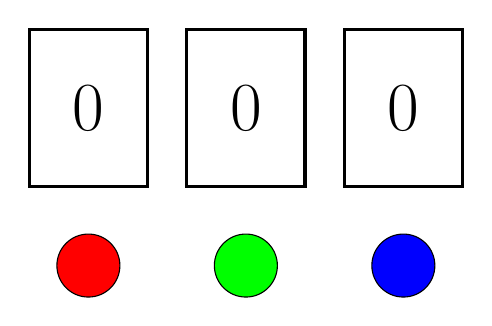
\begin{tikzpicture}
  % Kotak tampilan angka
  \foreach \x in {0,1,2} {
    \draw[very thick] (\x*2,2) rectangle ++(1.5,2);
    \node at (\x*2 + 0.75,3) {\Huge 0};
  }

  % Tombol
  \draw[fill=red] (0.75,1) circle (0.4);
  \draw[fill=green] (2.75,1) circle (0.4);
  \draw[fill=blue] (4.75,1) circle (0.4);
\end{tikzpicture}
\end{center}

Mesin ini memiliki cara kerja yang unik. Penekanan satu kali tombol biru akan menaikkan nilai digit satuan pada nomor urut, penekanan dua kali tombol hijau akan menaikkan nilai digit puluhan pada nomor urut, penekanan tiga kali tombol merah akan menaikkan nilai digit ratusan pada nomor urut, sebagai contoh:
\begin{itemize}
    \item Tombol biru ditekan satu kali akan menghasilkan nomor urut 001
    \item Tombol biru ditekan satu kali dan hijau dua kali menghasilkan nomor urut 011
    \item Tombol biru ditekan satu kali, hijau satu kali, dan merah tiga kali menghasilkan nomor urut 101
\end{itemize}

Jika penekanan tombol melebihi nilai pada masing-masing digit (0-9) maka angka yang ditampilkan pada digit tersebut akan dimulai dari awal lagi (RESET), sebagai contoh jika penekanan tombol biru dilakukan sepuluh kali, maka angka yang dihasilkan adalah 000.

    \item Jika dilakukan penekanan tombol secara berurutan merah $3^{2023}$ kali, hijau $2^{2024}$ kali, dan biru $5^{2025}$ kali, nomor urut berapa yang ditampilkan mesin? \textit{(Tuliskan jawaban dalam bentuk ANGKA saja)}

    \item Manakah konfigurasi penekanan tombol secara berurutan di bawah ini yang tidak mungkin menghasilkan angka 356?
    \begin{enumerate}
        \item MMMHHHHHHHMMMMHHHHHHBBBBBBBBMM
        \item MMMHHMMHHMMHHMMHHMMHHMMHHBBBBBB
        \item MMMHHHHHHHMMMMHHHHHHBBBBBBBBBBB
        \item MMMBHHBMBMHMBMBHMHMHMHMBMB
        \item MMMBHBHBHBHBHMHMHMHMHMHMB
    \end{enumerate}

\subsection*{Pohon Usia [22-23]}

\begin{center}
\begin{forest}
for tree={
  circle, draw, minimum size=7mm, inner sep=2pt, s sep=7mm, l sep=15mm, anchor=north,
}
[1
  [2, edge label={node[midway,left]{3}}
    [4, edge label={node[midway,left]{5}}
      [13, edge label={node[midway,left]{4}}]
      [14, edge label={node[midway,right]{3}}]
    ]
    [5, edge label={node[midway,right]{2}}
      [15, edge label={node[midway,left]{10}}]
      [16, edge label={node[midway,right]{6}}]
    ]
  ]
  [3, edge label={node[midway,right]{9}}
    [6, edge label={node[midway,right]{7}}
      [11, edge label={node[midway,left]{5}}
        [7, edge label={node[midway,left]{7}}]
        [8, edge label={node[midway,right]{1}}]
      ]
      [9, edge label={node[midway,right]{8}}
        [10, edge label={node[midway,left]{6}}]
        [12, edge label={node[midway,right]{4}}]
      ]
    ]
  ]
]
\end{forest}
\end{center}

Di kandang bebeknya Pak Tirta ada 16 bebek yang ia pelihara. Gambar di atas menunjukkan pengurutan bebek dari yang tertua hingga yang termuda. Angka di tepi antar simpul menunjukkan perbedaan usia antar dua bebek.  
Misalnya: bebek ke-6 lebih tua 8 tahun dari bebek ke-9.


    \item Tentukan berapa selisih usia Bebek 15 dan Bebek 7!  
    \textit{(Tuliskan jawaban dalam bentuk ANGKA saja)}

    \item Jika diketahui usia bebek ke-16 adalah 10 tahun, berapakah usia bebek ke-8?  
    \textit{(Tuliskan jawaban dalam bentuk ANGKA saja)}

\subsection*{Kirei [9-10]}

Perhatikan fungsi-fungsi berikut!

\begin{minted}{cpp}
int koi[10] = {12, 5, 6, 19, 2, 11, 26, 20, 4, 15};

int kirei() {
    int x = 0;
    for (int i = 0; i < 10; i++) {
        for (int j = 1; j*j < koi[i]; j++) {
            x += koi[i]/j;
        }
    }
    return x;
}
\end{minted}
    
    \item Tentukan nilai keluaran dari pemanggilan fungsi \texttt{kirei()}! \\
    Jawaban: \rule{4cm}{0.4pt} \textbf{\{Masukkan ANGKA saja tanpa SPASI\}}

    \item Anggap, nilai dari tiap bilangan bulat dalam array \texttt{koi} diperbesar menjadi dua kali lipat nilai sebelumnya. Lalu, fungsi \texttt{kirei()} dipanggil kembali dan dianggap nilai keluarannya adalah $a$. Jika jawaban dari soal sebelumnya dianggap sebagai $b$, tentukan hasil dari $\lfloor a/b \rfloor$! \\

    \textit{Catatan:} $\lfloor x \rfloor$ adalah fungsi yang mengeluarkan bilangan bulat paling besar yang lebih kecil atau sama dengan $x$. Sebagai contoh, keluaran dari $\lfloor 3.9133 \rfloor$ adalah 3.\\
    Jawaban: \rule{4cm}{0.4pt} \textbf{\{Masukkan ANGKA saja tanpa SPASI\}}




\end{enumerate}
\end{document}